\documentclass[a4paper,12pt]{article}
\usepackage[T1]{fontenc}
\usepackage[lmargin=0.5in,rmargin=0.5in,tmargin=0.6in,bmargin=0.6in]{geometry}

\usepackage{wrapfig}
\usepackage{graphicx}
\usepackage{xcolor}
\usepackage[hidelinks]{hyperref}

\begin{document}
\begingroup
\begin{center}
\LARGE \textbf{Curriculum Vit\ae}
\end{center}
\endgroup

\vspace{5pt}

\begingroup
\begin{center}
\large \textbf{Riccardo Bonalli}
\end{center}
\endgroup

\vspace{30pt}

\noindent\rule{18.5cm}{0.4pt}

\vspace{15pt}

\begin{wrapfigure}{r}{0.2\textwidth}
\centering
\hspace{-75pt}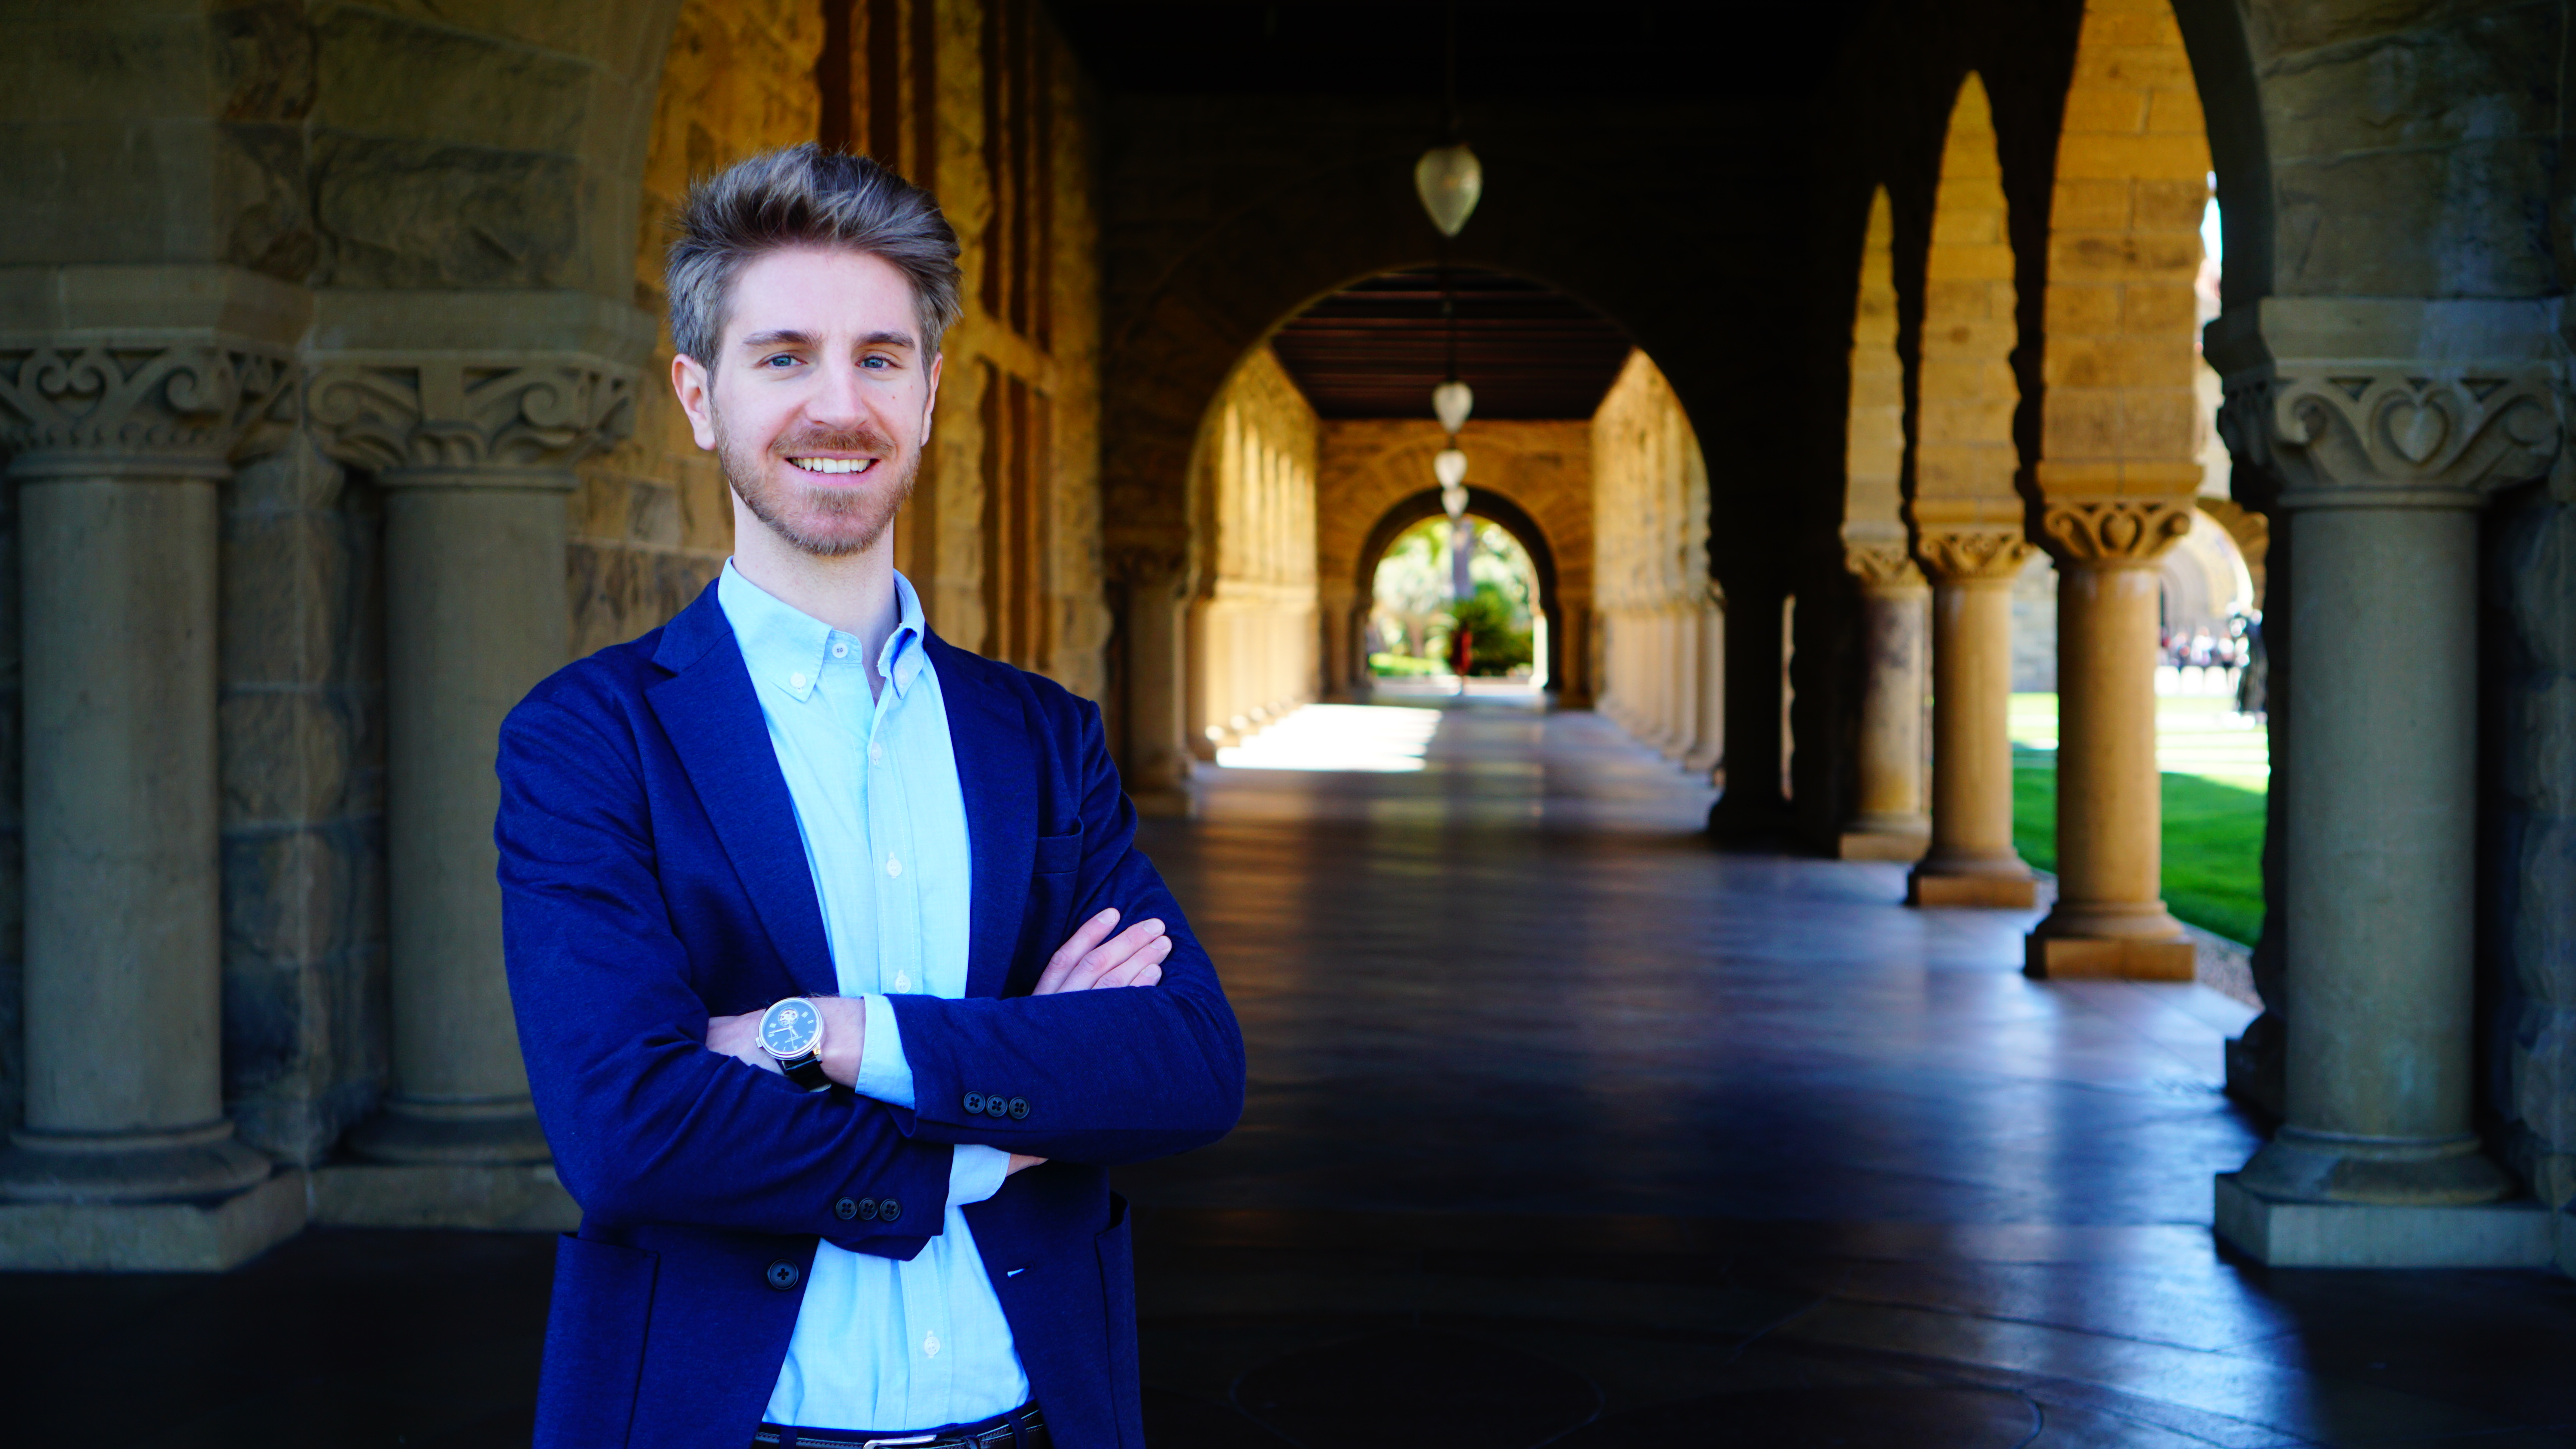
\includegraphics[width=0.3\textwidth]{pic}
\end{wrapfigure}

Born the 19th November 1989 in Varese (Italy) \\

Ph.D. Applied Mathematics \\

Postdoctoral Researcher

Autonomous Systems Laboratory (ASL)

Stanford Aeronautics \& Astronautics \\

William F. Durand Building,

496 Lomita Mall, Stanford, CA 94305-4035 \\

rbonalli@stanford.edu

\url{https://rbonalli.github.io}

\vspace{10pt}

\noindent\rule{18.5cm}{0.4pt}

\vspace{30pt}

\section{Academic Positions}
\begin{itemize}
\item From 07/2018: Postdoctoral Researcher at the Autonomous Systems Laboratory (Director Prof. Marco Pavone), Aeronautics \& Astronautics Department at Stanford University (USA), under a  NASA Early Career Faculty Grant.
\end{itemize}

\begingroup
\begin{center}
\noindent\rule{7cm}{0.4pt}
\end{center}
\endgroup

\section{Education}
\begin{itemize}
\item 04/2015-07/2018: Ph.D. in Applied Mathematics, Sorbonne Universit\'{e}, Paris (France). Collaboration between ONERA - The French Aerospace Lab and Laboratoire Jacques-Louis Lions. Advisors: Prof. Emmanuel Tr\'{e}lat (Sorbonne Universit\'{e}) and Dr. Bruno H\'{e}riss\'{e} (ONERA).
\item 09/2012-12/2014: MSc in Mathematical Engineering, Politecnico di Milano, Milan (Italy). Graduated with 111.75/110. Total SCH:  245/200.
\item 09/2008-09/2011: BSc in Physical Engineering, Politecnico di Milano, Milan (Italy).
\item 2008: Scientific High-School Diploma, Liceo Scientifico "Sereni", Luino (Italy).
\end{itemize}

\begingroup
\begin{center}
\noindent\rule{7cm}{0.4pt}
\end{center}
\endgroup

\section{Awards and Distinctions}
\begin{itemize}
\item 2018 : Best Ph.D. thesis at ONERA - TIS Department.

\url{https://www.onera.fr/fr/rejoindre-onera/prix-des-doctorants} (French)
\end{itemize}

\begingroup
\begin{center}
\noindent\rule{7cm}{0.4pt}
\end{center}
\endgroup

\section{Research Interests}

My research activities concern infinite dimensional optimization, control and mechanical systems theory, theoretical and numerical reinforcement learning and their applications to robust and optimal control. I am particularly interested in leveraging information from theoretical analysis of problems to design efficient numerical algorithms, mainly for a real-time computations of optimal strategies. During my Ph.D., I specialized in optimal control problems in aerospace such as endo/exo-atmospheric rendezvous and motion planning in aeronautics, and I also provided state-of-the-art C++ based softwares for fast predictions of missile interception missions. During my postdoc at the Department of Aeronautics \& Astronautics at Stanford University, I am focusing on several topics: theoretical and numerical developments for sequential convex programming, path-planning and human-robot interaction, Riemannian Motion Control Policy (RMCP) and reinforcement learning procedures. The main objective consists of computing robust optimal controls in real time for freeflyer systems and robotic manipulators. These algorithms will be tested on real challenging scenarios by NASA on the International Space Station (ISS), starting from September 2019. I have recently started to adapt such paradigms to solve different problems, such as, high-dimensional Autonomous Mobility on Demand (AMoD). \\

\begin{itemize}
\item \textbf{Infinite Dimensional Optimization:} variational principles, convex analysis in Banach spaces, Lagrange multiplier rules for nonlinear constrained optimization problems.
\item \textbf{Finite Dimensional Control Theory:} Riemannian and symplectic geometry applied to geometric control, dynamical systems theory, maximum principles, high order necessary and sufficient optimality conditions, optimal control problems with control and state constraints, optimal control problems with delays in the state and in the control.
\item \textbf{Analysis of Numerical Methods for Optimal Control:} sequential convex and quadratic programming, MPC, shooting and multi-shooting methods for optimal control problems with state constraints and delays, numerical homotopy and continuation methods, motion planning and RMCP with application to human-robot interaction, theoretical and numerical analysis of reinforcement learning algorithms applied to optimal control.
\item \textbf{Applications:} real-time optimal control of launch vehicle systems involved in rendezvous problems, atmospheric reentry and satellite orbit transfert, real-time optimal control of freeflyer and robotic manipulators for sensitive operations on the ISS, fast computations of optimal solutions for massive AMoD problems.
\end{itemize}

\begingroup
\begin{center}
\noindent\rule{7cm}{0.4pt}
\end{center}
\endgroup

\section{Publications}

\subsection{Preprint and Work in Progress Papers}

\begin{enumerate}
\item M. Szmuk, D. Malyuta, \textbf{R. Bonalli}, B. A\c{c}ıkme\c{s}e and M. Pavone, \textit{Convex-based Methods for Trajectory Optimization}. Work in progress to submit to IEEE Control Systems Magazine.
\item A. Bylard, \textbf{R. Bonalli} and M. Pavone, \textit{Riemannian Control Policies and Second-Order Riemannian Motion Policies for Scalable and Modular Geometric Control}. Work in progress to submit to the International Conference on Robotics and Automation, 2020, Paris (France).
\end{enumerate}

\subsection{Journal Papers}

\begin{enumerate}
\item \textbf{R. Bonalli}, B. H\'{e}riss\'{e} and E. Tr\'{e}lat. \textit{Optimal Control of Endo-Atmospheric Launch Vehicle Systems: Geometric and Computational Issues}. IEEE Transaction on Automatic Control (To appear, 2020). \url{https://arxiv.org/abs/1710.11501}
\item \textbf{R. Bonalli}, B. H\'{e}riss\'{e} and E. Tr\'{e}lat. \textit{Continuity of Pontryagin Extremals with Respect to Delays in Nonlinear Optimal Control}. SIAM J. Control Optim., 57 (2019), pp. 1440--1466. \url{https://epubs.siam.org/doi/abs/10.1137/18M119121X}
\end{enumerate}

\subsection{Conference Papers}

\begin{enumerate}
\item \textbf{R. Bonalli}, A. Cauligi, A. Bylard, T. Lew and M. Pavone, \textit{Trajectory Optimization on Manifolds: A Theoretically-Guaranteed Embedded Sequential Convex Programming Approach}. Robotics: Science and Systems, 2019, Freiburg (Germany). \url{https://arxiv.org/abs/1905.07654}
\item \textbf{R. Bonalli}, A. Cauligi, A. Bylard and M. Pavone, \textit{GuSTO: Guaranteed Sequential Trajectory Optimization via Sequential Convex Programming}. International Conference on Robotics and Automation, 2019, Montreal (Canada). \url{https://arxiv.org/abs/1903.00155}
\item \textbf{R. Bonalli}, B. H\'{e}riss\'{e}, H. Maurer and Emmanuel Tr\'{e}lat. \textit{The Dubins Car Problem with Delay and Applications to Aeronautics Motion Planning Problems}. 18th French - German - Italian Conference on Optimization, 2017, Paderborn (Germany).
\item \textbf{R. Bonalli}, B. H\'{e}riss\'{e} and E. Tr\'{e}lat. \textit{Analytical Initialization of a Continuation-Based Indirect Method for Optimal Control of Endo-Atmospheric Launch Vehicle Systems}. IFAC World Congress, 2017, Toulouse (France). \url{https://www.sciencedirect.com/science/article/pii/S2405896317301283}
\item \textbf{R. Bonalli}, B. H\'{e}riss\'{e} and E. Tr\'{e}lat. \textit{Solving Optimal Control Problems for Delayed Control-Affine Systems with Quadratic Cost by Numerical Continuation}. American Control Conference, 2017, Seattle (USA). \url{https://ieeexplore.ieee.org/document/7963026}
\end{enumerate}

\subsection{Ph.D. Thesis}

\begin{itemize}
\item \textbf{R. Bonalli}, \textit{Optimal Control of Aerospace Systems with Control-State Constraints and Delays}. Defended on July 13, 2018 (Sorbonne Universit\'e). Dissertation committee: Jean-Baptiste Caillau, Jean-Michel Coron, Bruno H\'eriss\'e, Nicolas Petit, Jean-Baptiste Pomet, Emmanuel Tr\'elat and Hasnaa Zidani. \url{https://tel.archives-ouvertes.fr/tel-01848542v3/document}
\end{itemize}

\begingroup
\begin{center}
\noindent\rule{7cm}{0.4pt}
\end{center}
\endgroup

\section{Workshops}

\begin{itemize}
\item \textit{Space Robotics}. Robotics: Science and Systems, 2019, Freiburg (Germany). Organizers: \textbf{R. Bonalli}, M. Pavone, N. Ahmed, D. Szafir, C. Heckman, J. McMahon and E. Komendera.
\end{itemize}

\begingroup
\begin{center}
\noindent\rule{7cm}{0.4pt}
\end{center}
\endgroup

\section{Invited Lectures and Talks}

\begin{itemize}
\item May 24, 2019, \textit{Real-time Optimal Control of Robotics Systems}. Talk at Concordia University, Montreal (Canada).
\item May 15, 2019, \textit{Real-time Optimal Control of Endo-Atmospheric Launch Vehicles}. Informal Systems Seminar at McGill University, Montreal (Canada).
\item October 1, 2018, \textit{Methods for Real-time Optimal Guidance of Launch Vehicles}. Ph.D. Students Welcome Day at ONERA - The French Aerospace Lab, Palaiseau (France).
\end{itemize}

\begingroup
\begin{center}
\noindent\rule{7cm}{0.4pt}
\end{center}
\endgroup

\section{Software and Hardware Experiments}

\begin{itemize}
\item \texttt{GuSTO} - Julia package implementing GuSTO, a sequential convex programming paradigm for real-time trajectory optimization. Developed in collaboration with Andrew Bylard and Abhishek Cauligi during my Postdoc at Stanford University, this library combines ease-of-use with fast computations, providing solutions in real-time for many robotic systems. The open source code is available at: \url{https://github.com/StanfordASL/GuSTO.jl}.
\item \texttt{SOCP} - C++ package implementing shooting for optimal control problems, specialized in launch vehicles. This paradigm has been developed during my Ph.D thesis in collaboration with Bruno H\'eriss\'e and it can compute optimal solutions for aerospace rendezvous problems in few milliseconds. A (partial) open source version is available at: \url{https://github.com/bherisse/socp}.
\item Freeflyer experiments on simulated two-dimensional micro-gravity environment at Stanford University, in collaboration with Andrew Bylard and Abhishek Cauligi. The video is available at: \url{https://www.youtube.com/watch?v=GHehE-If5nY}.
\item \texttt{Astrobee} - Real-time optimal control of the NASA robot Astrobee via GuSTO (in collaboration with Andrew Bylard and Abhishek Cauligi). Experiments considering sensitive operations on the International Space Station have been conducted in Summer 2019.
\end{itemize}

\begingroup
\begin{center}
\noindent\rule{7cm}{0.4pt}
\end{center}
\endgroup

\section{Teaching Activity}

\subsection{Graduate Courses}

\begin{itemize}
\item Spring 2019: Teaching assistant for the course \textit{Optimal and Learning-Based Control (AA203)} held at Stanford University by Prof. Marco Pavone.
\end{itemize}

\subsection{Senior Undergraduate Courses}

\begin{itemize}
\item 2015-2017: Teaching assistant for the course \textit{Analysis and Stability of Dynamical Systems (AO102)} held at ENSTA ParisTech by Prof. Fr\'{e}d\'{e}ric Jean.
\item 2016-2017: Teaching assistant for the course \textit{Quadratic Optimization (AO101)} held at ENSTA ParisTech by Prof. Hasnaa Zidani.
\end{itemize}

\begingroup
\begin{center}
\noindent\rule{7cm}{0.4pt}
\end{center}
\endgroup

\section{Student Supervision}

\subsection{Ph.D. Students}

\begin{itemize}
\item Andrew Bylard, Stanford University, from 08/2018 (at 50\%).

Ph.D. student in control for aerospace and robotics systems at Stanford University. 
\end{itemize}

\subsection{Master Students}

\begin{itemize}
\item Quentin Chan-Wai-Nam, MINES ParisTech, 03/2017-08/2017 (at 30\%).

Master thesis for the MSc in automatic and control. Title: \textit{Predictive Control Methods by Shooting Algorithms}.
\end{itemize}

\begingroup
\begin{center}
\noindent\rule{7cm}{0.4pt}
\end{center}
\endgroup

\section{Industrial Experiences}

\begin{enumerate}
\item 03/2015 - 07/2018: Ph.D. thesis at ONERA - The French Aerospace Lab, Paris (France).

Design of onboard methods for real-time computing of optimal strategies for launch vehicle systems. ONERA owns a software based on the latest version of my algorithm.
\item 2014: MSc Internship at IFP Energies Nouvelles, Paris (France).

Six months of internship from March 2014 to August 2014 consisting of the improvement of algorithms inside a C++ thermodynamics library using
different nonlinear optimization techniques.
\end{enumerate}

\begingroup
\begin{center}
\noindent\rule{7cm}{0.4pt}
\end{center}
\endgroup

\section{Computer Skills}

\begin{itemize}
\item Operating Systems: UNIX (Scientific Linux, Ubuntu), Mac OS, Windows.
\item Programming Languages : GNU Bash, CMake, C, C++, Fortran90, Python, Julia, \LaTeX.
\item Softwares: MatLab, FreeFem++, Microsoft Office.
\end{itemize}

\begingroup
\begin{center}
\noindent\rule{7cm}{0.4pt}
\end{center}
\endgroup

\section{Others}

\begin{itemize}
\item Languages: italian (mothertongue), english (fluent), french (fluent).
\item Sports: rowing and judo (for which I participated in regional competitions), swimming, climbing and down-hill.
\item Music: piano and classical guitar.
\item Interests: viticulture, history, philosophical politics and politics.
\end{itemize}

\end{document}